\label{section_models}
\section{Maze and multi-agent exploration}
\label{section_models_maze}
For simulation purposes, this work used an open-source tool that models a maze under a 4-neighbor 2D grid graph perspective, where each cell is a square with its edges composed by a wall or not. If there is a wall, an agent cannot traverse the maze through the corresponding edge. On the other hand, if there is not a wall, an agent has a free way to traverse the maze through the related edge. It is worth to mention that, if an edge has a wall, the edge of the adjacent corresponding cell also has necessarily a wall. Likewise, if an edge has not a wall, the edge of the adjacent corresponding cell doesn't have a wall.

The maze has a goal that is a single marked cell, and an agent inside the maze aims to find the marked cell, traversing the maze cell by cell. This agent is an autonomous entity that follows a specific algorithm and previously programmed rules. So that it doesn't go through the same path more than one time, it stores the visited cells. Thus, when there are various possible branches to extend the agent's path, it ignores cells already visited by itself. If there is no candidate to be a possible branch, the agent goes back to the previous visited cell. Furthermore, if more than one agent traverses the maze in order to find the goal, differently from some approaches presented in \citen{Beisel2014}, \citen{Burgard2005}, and \citen{KivelevitchCohen2010}, there is no intercommunication between agents in the approach of this research, i.e., an agent knows nothing about another agent's search.

\citen{Muhammad2021} developed an open-source maze generator. It is a python module that creates randomly mazes and enables the user to simulate its own maze-solving algorithm. In this context, this work presents a multi-agent maze-solving algorithm that has been simulated over \citen{Muhammad2021} open-source code, with modifications. Figure \ref{maze_model} presents, for example, 2 agents traversing a $6 \times 6$ maze toward the goal.

\citen{Muhammad2021} software creates by default a ``perfect maze'', which means that there is one and only one path to the goal from any cell. However, it is possible to set the code to generate a imperfect maze.

\begin{figure}[ht!]
\centering
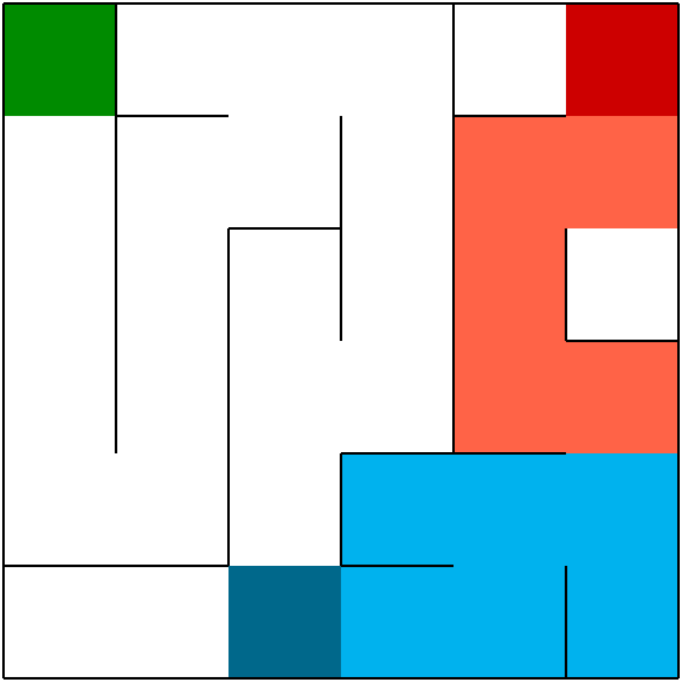
\includegraphics[width=0.5\textwidth]{Cap2/maze_model.png}
\caption{Blue and red agents traversing a $6\times 6$ maze. The goal is represented by the green entity. This maze is a perfect maze \cite{Muhammad2021}.}
\label{maze_model}
\end{figure}

\section{Maze from a graph topology perspective}
\label{section_models_maze_graph}
As pointed out in Section \ref{section_models_maze}, given that an agent ignores visited cells, there are important statements related to this work:

\begin{itemize}
\item if there is only one path to the goal from any cell, it is valid to consider a maze as a tree, i.e., a perfect maze \cite{Muhammad2021};

\item if there is more than one path to the goal from any cell, the maze cannot be considered as a tree, but it might be considered as a general 2D grid;

\item regarding the last statement, even though not every maze can be considered as a tree, an agent path might be individually interpreted as a tree if such agent does not go through already visited cells, except in backtracking situations.
\end{itemize}

Figure \ref{maze_example_graph} gives an example of the graph representation of the maze presented in Figure \ref{maze_example}, where a red agent is traversing the maze toward the green goal. As established by \citen{Muhammad2021}, the maze cells are programmatically addressed as indices of a matrix, such as represented in Figure \ref{maze_indices_muhammad}.

\begin{figure}[ht!]
\centering
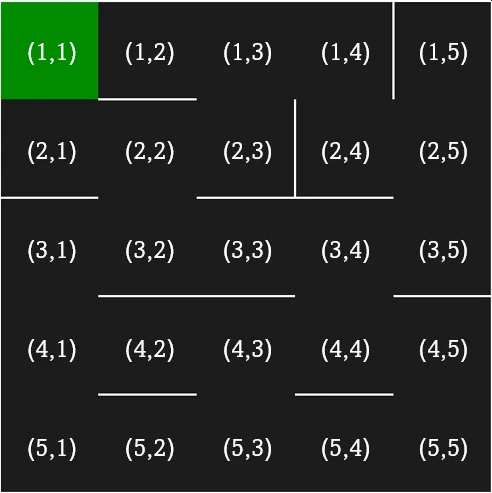
\includegraphics[width=0.5\textwidth]{Cap2/maze_indices_muhammad.png}
\caption{Maze cell indices. Source: \citen{Muhammad2021}.}
\label{maze_indices_muhammad}
\end{figure}

\begin{figure}
    \centering
    \subfloat[\centering Agent at starting cell]
    {{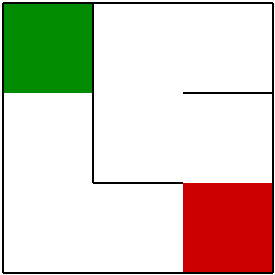
\includegraphics[width=3cm]{Cap2/maze_perfect_3x3_1agent_1.png} }}
    \qquad
    \subfloat[\centering Agent's 2nd step]
    {{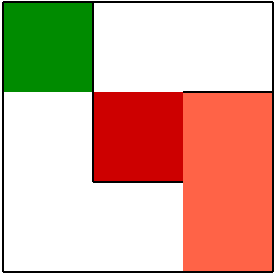
\includegraphics[width=3cm]{Cap2/maze_perfect_3x3_1agent_2.png} }}
    \qquad
    \subfloat[\centering Agent's 10th step]
    {{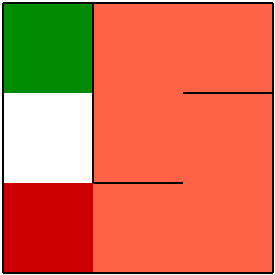
\includegraphics[width=3cm]{Cap2/maze_perfect_3x3_1agent_3.png} }}
    \caption{Red agent traversing a maze toward the green goal. This maze is a perfect maze \cite{Muhammad2021}.}
    \label{maze_example}
\end{figure}

\begin{figure}[ht!]
\centering
\begin{forest}
 [3 3,for tree={circle,draw},s sep=12mm,fill=red!100
 	[2 3
 		[2 2
 			[1 2
 				[1 3]]]]
 	[3 2
 		[3 1
 			[2 1
 				[1 1,fill=green!100]]]]]
\end{forest}
\caption{Graph representation of the maze presented in Figure \ref{maze_example}. The cell indices are pointed out. The agent starts at index (3,3), and achieves the goal at index (1,1).}
\label{maze_example_graph}
\end{figure}



\section{Multi-agent exploration without communication}
\label{section_models_exploration}
\subsection{Our algorithm's key concepts}
\label{section_models_exploration_key_concepts}
The goal of this work is to present a maze-solving algorithm in a multi-agent environment, where an agent cannot communicate with the other agents. Thus, each agent must be previously programmed to avoid exploring the same portion of the maze as other agents. Indeed, they should be as dispersed as possible.

First of all, this research considers a maze as a graph, where each node is a cell representing the maze. Given an initial node from which the agent starts its path, the agent checks if the node has children. Since the graph is undirected, i.e., there are no completely walled cells, this work establishes some statements:

\begin{itemize}
\item if an agent finds the cell where the goal is, the agent finishes its path;

\item if an agent is not in the cell where the goal is and the cell has only one unwalled edge, the agent necessarily goes through such edge;

\item if an agent is not in the cell where the goal is and the cell has more than one unwalled edge, the agent needs to decide which edge it will go through.
\end{itemize}

To establish a decision algorithm to the last statement, this work proposes firstly an interval division related to the agents and the nodes around them. Supposing that there are $k$ agents $a_{1}, a_{2},...,a_{k}$ to explore the maze, each agent will have a corresponding and proportional range of action related to the graph, as presented below:

\begin{equation}
\label{equation_agent_intervals}
	\begin{align}
			d = 1/k\\
		a_{1} \textnormal{: } [0, d[\\
		a_{2} \textnormal{: } [d, 2d[\\
		a_{3} \textnormal{: } [3d, 4d[\\
		...\\
		a_{k} \textnormal{: } [(k-1)d, 1]
	\end{align}
\end{equation}
where $d$ is the size of the partition corresponding to each agent. On the other hand, this work has handled convergence intervals to each node, where the agents tends to match its interval with the node's convergence interval. In this way, an agent intends to traverse the maze as dispersed from the others as possible.

To disperse the agents through the maze, this work establishes some steps in order to guide the agent, that knows nothing about another agent's search. As a starting point for graph exploration, our algorithm works specifically in the context of perfect mazes \cite{Muhammad2021}. The following steps base the reasoning expressed in the proposed pseudocode in Section \ref{section_models_exploration_pseudocode}:

\begin{itemize}
\item every agent $a_{i}$ has a previously programmed interval;

\item every agent starts its search at the same cell, i.e., the root of an agent's tree is the same for any agent. The root's converge interval is $[0,1]$;

\item every agent explores the maze calculating dynamically the converge intervals of the children of the current node where the agent is. These convergence intervals are calculated based on the following steps:

	\begin{itemize}

	\item if there is only one child, the child's convergence interval is the same as the current node's convergence interval;
	
	\item if there is more than one child, the current node's convergence interval is uniformly split between its children;
	
	\end{itemize}
	
\item every agent must go to the first child that its convergence interval intersects the agent's interval. The order of children must be well defined so that every agent gets the same calculation result of some node's convergence interval. Then, in the context of perfect mazes, it ensures that every cell (node) has the same convergence interval regardless of the agent. This research established a clockwise order for the cells - North, East, South, West - from left to right regarding the insertion of children;

\item an agent doesn't visit an already visited node, except in backtracking situations where there are no children to visit, i.e., the node in fact has no children, the children have already been visited, or there are no more children that match its convergence intervals to the agent's interval;

\item every agent must fill its interval going through the correspondent nodes until finds the goal. If it doesn't find the goal, but it fills its interval, surely the convergence interval of the goal node is outside of the agent's interval. In this context, the agent stops the search or changes its decision algorithm. In the case that it changes its behavior, this work proposes two optional secondary conducts:

	\begin{itemize}

	\item the agent modifies its interval and the exploration order from left-right to right-left. Section \ref{section_results} discusses broader about this point;
	
	\item the agent explores the maze using some DFS algorithm, but ignores already visited nodes.
	
	\end{itemize}
\end{itemize}

The following pictures expose key concepts of our algorithms:

\begin{itemize}

\item Figure \ref{maze_example_graph_dispersion} is related to the dispersion concept, in which every agent explores the maze as dispersed as possible from another agent;
	
\item Figure \ref{maze_example_graph_intervals} presents the convergence intervals of the cells (nodes) of a fictional maze when a given agent explores it based on the aforementioned steps;

\item Figure \ref{maze_example_graph_ignoring_big_trees} exposes an agent with an interval $[0,\frac{1}{2}[$ prioritizing to fill completely its interval, despite there being a bigger subtree on the right of the root. In fact, our algorithm is an exploration algorithm, so an agent has no information about the structure of the maze. It is worth to emphasizing that when an agent finishes its interval, it needs to change its behavior or simply stop the search;

\item Figure \ref{maze_example_graph_mandatory_stop} exposes the visit order of an agent with interval $[\frac{1}{3},\frac{2}{3}[$. Due to the fact that the agent finishes its interval in the 7th visited node, and it doesn't go through already visited nodes, except in backtracking situations, it never finds the green goal, regardless of the behavior that it assumes after finishing its interval. Therefore, an agent might be unsuccessful in the search because it doesn't repeat a crossing - from a node to another node in the same direction - more than one time.
	
\end{itemize}

\begin{figure}[ht!]
\centering
\begin{forest}

%for tree={circle,draw,minimum size=3em,inner sep=1pt,s sep=12mm}

 [root,label=above:{\textit{Starting point}},for tree={circle,draw,minimum size=2em}
 	[,for tree={fill=red!100}
 		[
 			[]
 			[]]
 		[
 			[]
 			[]]]
 	[,for tree={fill=blue!100}
 		[
 			[]
 			[]]
 		[
 			[]
 			[]]]
 	[,for tree={fill=yellow!100}
 		[
 			[]
 			[]]
 		[
 			[]
 			[]]]]

\end{forest}
\caption{Three agents (Red, Blue, and Yellow) disperse from each other in a fictional and perfect maze.}
\label{maze_example_graph_dispersion}
\end{figure}

\begin{figure}[ht!]
\centering
\begin{forest}

%for tree={circle,draw,minimum size=3em,inner sep=1pt}

 [root,label=above:{\textit{Starting point}},for tree={circle,draw,s sep=12mm,minimum size=2em},label=below:{$[0,1]$}
 	[,label=below:{$[0,\frac{1}{2}[$}
 		[,label=below:{$[0,\frac{1}{4}[$}
 			[,label=below:{$[0,\frac{1}{8}[$}]
 			[,label=below:{$[\frac{1}{8},\frac{1}{4}[$}]]
 		[,label=below:{$[\frac{1}{4},\frac{1}{2}[$}]]
 	[,label=right:{$[\frac{1}{2},1[$}
 		[,label=below:{$[\frac{1}{2},1]$}
 		[,label=below:{$[\frac{1}{2},\frac{3}{4}[$}]
 		[,fill=green!100,label=below:{$[\frac{3}{4},1]$}]]]]

\end{forest}
\caption{A fictional maze represented as a tree where each node has an established interval according to an agent's traverse guided by Pseudocode \ref{pseudocode_1}. The green node represents the goal.}
\label{maze_example_graph_intervals}
\end{figure}

\begin{figure}[ht!]
\centering
\begin{forest}

%for tree={circle,draw,minimum size=3em,inner sep=1pt,s sep=12mm}

 [root,label=above:{\textit{Starting point}},for tree={circle,draw,minimum size=2em}
 	[,for tree={fill=red!100}
 		[]
 		[]]
 	[,for tree={fill=black!0}
 		[
 			[$\vdots$,for tree={draw=black!0}]
 			[
 				[$\vdots$,for tree={draw=black!0}]]]
 		[
 			[
 				[$\vdots$,for tree={draw=black!0}]
 				[$\vdots$,for tree={draw=black!0}]
 				[$\vdots$,for tree={draw=black!0}]]]
 		[
 			[$\vdots$,for tree={draw=black!0}]
 			[
 				[$\vdots$,for tree={draw=black!0}]
 				[$\vdots$,for tree={draw=black!0}]]]]]

\end{forest}
\caption{A red agent with an interval $[0,\frac{1}{2}[$ prioritizing to fill completely its interval in a fictional maze.}
\label{maze_example_graph_ignoring_big_trees}
\end{figure}

\begin{figure}[ht!]
\centering
\begin{forest}

%for tree={circle,draw,minimum size=3em,inner sep=1pt,s sep=12mm}

 [1,label=above:{\textit{Starting point}},for tree={circle,draw,minimum size=2em,s sep=12mm},label=below:{$[0,1]$},fill=red!100
 	[2,label=below:{$[0,\frac{1}{2}[$},fill=red!100
 		[,label=left:{$[0,\frac{1}{4}[$}
 			[$\vdots$,draw=black!0
 				[,fill=green!100]]]
 		[3,label=below:{$[\frac{1}{4},\frac{1}{2}[$},fill=red!100
 			[4,label=below:{$[\frac{1}{4},\frac{3}{8}[$},fill=red!100]
 			[5,label=below:{$[\frac{3}{8},\frac{1}{2}[$},fill=red!100]]]
 	[6,label=below:{$[\frac{1}{2},1]$},fill=red!100
 		[7,label=below:{$[\frac{1}{2},\frac{3}{4}[$},fill=red!100]
 		[,label=below:{$[\frac{3}{4},1]$}
 			[,label=below:{$[\frac{3}{4},\frac{7}{8}[$}]
 			[,label=below:{$[\frac{7}{8},1]$}]]]]

\end{forest}
\caption{An agent with interval $[\frac{1}{3},\frac{2}{3}[$ finishes its interval in the visit order indicated. Regardless of the behavior that it assumes after finishing its interval, it never finds the green goal since it doesn't go through already visited nodes, except in backtracking situations. It is a fictional maze.}
\label{maze_example_graph_mandatory_stop}
\end{figure}



\subsection{Pseudocode for our algorithm}
\label{section_models_exploration_pseudocode}

As pointed out in Section \ref{section_definitions_graph}, a graph may be represented as an adjacency list. Given that an agent path through an unknown maze may be represented as a tree in the situation approached in Section \ref{section_models_maze_graph}, where an agent does not go through already visited cells, except in backtracking situations, and considering the agent path as an adjacency list $A$, where the first explored node (root) $v_{1}$ has a convergence interval equal to $[0,1]$, while the other nodes $v_{i}$ of the maze are unknown, i.e., the agent doesn't know previously their convergence intervals, Pseudocode \ref{pseudocode_1} establishes the convergence intervals of each node specifically in the context of perfect mazes \cite{Muhammad2021}, despite being a starting point to solve similar problems in the context of imperfect mazes, i.e., the graph of the maze cannot be considered as tree in a macro view.

As mentioned previously, there is no communication between agents. Therefore, Pseudocode \ref{pseudocode_1} considers that each agent needs to explore the maze individually and calculate by itself the convergence intervals of each node. Furthermore, it is important to emphasize that each agent considers individually the maze as tree, where the root is the agent's starting node.

\begin{algorithm}
\caption{Traverse of the agent through the maze (interpreted as a tree by the agent).}
\label{pseudocode_1}
\begin{algorithmic}%[1]
\State /* \textit{Previously defined interval of the agent} */

\State agent\_interval $\gets$ $[a_{min},a_{max}[$

\State

\State /* \textit{Agent starts the exploration at node $v_{1}$} */

\State current\_node $\gets$ $v_{1}$

\State

\State /* \textit{Array of visited nodes by the agent is initially empty} */

\State visited\_nodes $\gets [$ $ ]$

\State

\State /* \textit{$v_{1}$ is the root, so its interval comprises the entire range of visits} */

\State intervals$[v_{1}] \gets [0,1]$

\State

\State /* \textit{Initialize the empty adjacency list of the tree $A$} */

\State $A \gets \oslash$

\State

\State /* \textit{In the tree $A$, create a node for $v_{1}$, and fill its children list with the neighboring cells of $v_{1}$. The children insertion order must follow some immutable rule. In the case of this work, the insertion is clockwise (North, East, South, West)} */

\State complete$(A, v_{1})$

\State

\State /* \textit{Create a flag to know if the agent filled its interval passing by all the correspondent nodes in the tree} */

\State finished\_interval $\gets$ FALSE

\State

\State

\While{current\_node \textit{is not the goal cell}}

\If{current\_node \textit{has no child} \textbf{or} \textit{all of} current\_node'\textit{s children were visited}}

\If{current\_node == $v_{1}$} \Comment{\textit{Unsuccessful search}}

\State \textbf{break} 

\Else

\State current\_node $\gets$ get\_parent(A, current\_node)

\State \textbf{continue}

\EndIf

\EndIf

\If{current\_node \textit{is not in} visited\_nodes}

\State append(visited\_nodes, current\_node)

\State max $\gets$ get\_max\_value(intervals[current\_node])

\State min $\gets$ get\_min\_value(intervals[current\_node]) \Comment{\textit{Node's mixed radix value}}

\State partition $\gets$ (max - min) \slash amount\_of\_children

\State count $\gets$ 0

\ForAll{child $v_{j}$ of current\_node in $A$}

\State intervals[$v_{j}$] $\gets$ [min + count $\cdot$  partition, min + (count+1) $\cdot$  partition[

\State complete(A, $v_{j}$)

\State count $\gets$ count + 1

\EndFor

\EndIf

\algstore{alg1}

\end{algorithmic}
\end{algorithm}

\begin{algorithm}
\ContinuedFloat
\caption{Traverse of the agent through the maze (interpreted as a tree by the agent).}
\begin{algorithmic}%[1]
\algrestore{alg1}

\ForAll{\textit{child} $v_{j}$ \textit{of} current\_node \textit{in} $A$}

\State max\_node $\gets$ get\_max\_value(interval[$v_{j}$])

\State min\_node $\gets$ get\_min\_value(interval[$v_{j}$])

\State max\_agent $\gets$ get\_max\_value(agent\_interval)

\State min\_agent $\gets$ get\_min\_value(agent\_interval)

\If{$v_{j}$ \textit{is in} visited\_nodes}

\State \textbf{continue}

\ElsIf{max\_agent < min\_node}

\State /* \textit{If the node's interval is on the right of the agent's interval, surely the}
\State \textit{agent has finished its interval. Since the order of the nodes are well defined,}
\State \textit{and in increasing order of intervals, the following condition improve the}
\State \textit{algorithm's performance. It is optional} */

\State finished\_interval $\gets$ TRUE

\State \textbf{break}

\ElsIf{min\_agent < max\_node \textbf{and} max\_agent > min\_node}

\State /* \textit{This condition verifies if there is intersection between the agent's interval}
\State \textit{and the node's interval. The order of children must be well defined} */

\State current\_node $\gets v_{j}$

\State \textbf{break}

\EndIf

\EndFor

\State

\State /* \textit{If} current\_node \textit{remains the same as it was at the beginning of the iteration,}

\State \textit{and it is the root, the agent has finished its interval} */

\If{current\_node == $v_{1}$ \textbf{and} finished\_interval == FALSE}

\State finished\_interval $\gets$ TRUE

\EndIf

\State

\State /* \textit{If the agent completely filled its interval, it needs to change its behavior, since its}
\State \textit{behavior is domain dependent. It might continue the DFS under some criteria.}
\State \textit{Otherwise, it must come back to parent in order to verify if there are more nodes to}
\State \textit{visit} */

\If{finished\_interval == TRUE}

\State current\_node $\gets$ continue\_DFS\_under\_some\_criteria(A, current\_node)

\Else

\State current\_node $\gets$ get\_parent(A, current\_node)

\EndIf

\EndWhile

\end{algorithmic}
\end{algorithm}

Thus, the goal of this work aims to establish an efficient algorithm that interrelates agent intervals to node convergence intervals. Furthermore, the authors observed that a mixed radix representation to the agents' path is a powerful mathematical tool for relating such path to the node's convergence interval that the agent is visiting. Section \ref{section_models_mixed_radix} discusses the mixed radix representation.

\section{Mixed radix representation to the agent path}
\label{section_models_mixed_radix}
In Section \ref{section_models_exploration}, this work presented a method for an agent to traverse the maze by defining ranges of action. Pseudocode \ref{pseudocode_1} exposes this method and establishes a way to explore the maze while an agent records the visited nodes and the explored tree. However, the agent doesn't need in fact to save all the structure of the tree, because it only needs to know the current node's convergence interval and the current node's edges to make a decision.

This work establishes a method to calculate the node's convergence intervals without the agent having to save necessarily all the structure of the tree. In order to traverse the maze while the agent autonomously makes a decision node by node, it saves its path in a mixed radix numerical representation, where the starting representation is ``$0.$'', and it is limited to 1, i.e., $[0,1]$. Pseudocode \ref{pseudocode_2} proposes a computational method to get the value of mixed radix numerical representation. Equation \ref{equation_mixed_radix_value_examples} shows examples of numbers under a mixed radix representation.

\begin{equation}
\begin{flalign}
& 0.0_{2}1_{2} = 0.25\\
& 0.0_{2}2_{3} = 0.333...\\ %1/3
& 0.0_{2}2_{3}1_{2} = 0.41666...\\ %5/12
& 0.1_{5}1_{3}0_{2}1_{2} = 0.28333...\\ %17/60
& 0.8_{9}2_{7}2_{3}2_{3}5_{8} \approx 0.93584656 %4245/4536
\end{flalign}
\label{equation_mixed_radix_value_examples}
\end{equation}

According to the order of analysis of the children and the mathematical tools to calculate node convergence intervals that are presented in Pseudocode \ref{pseudocode_1}, the items below present how the agent saves its path based on a mixed radix representation. These points guide the reasoning in Pseudocode \ref{pseudocode_2}.

\begin{itemize}
\item If the current node has only one child and the agent goes through this child, it appends $I_{1}$ to the mixed radix numerical representation of the path;

\item If the current node has $n$ children, where $n > 1$, and the agent decides to go through the \textit{i}th child, it appends $(i-1)_{n}$ at the end of the mixed radix numerical representation of the path;

\item If the agent must go back to the parent, it removes the last appended value from the mixed radix numerical representation of the path.
\end{itemize}

It is important to note that the value of the mixed radix numerical representation is the same as the minimum value of the convergence interval of the node that the agent is visiting. Moreover, the mixed radix numerical representation carries information about the maximum value of the node's convergence interval, since it is the sum of the minimum value with the lowest possible value of the current mixed radix representation. For instance, if the agent's current path is $0.1_{3}0_{2}2_{4}$, the minimum value of the current node's convergence interval is $0.1_{3}0_{2}2_{4}$, and the maximum is $0.1_{3}0_{2}3_{4}$ ($0.1_{3}0_{2}2_{4} + 0.0_{3}0_{2}1_{4}$). Figure \ref{mixed_radix_path_example} presents an example of the approach of a mixed radix numerical representation, where the agent's path carries information about the current node's convergence interval.

\begin{algorithm}
\caption{Methods related to mixed radix numerical representation.}
\label{pseudocode_2}
\begin{algorithmic}

\State /* \textit{Structure of mixed radix element} */

\State \textbf{struct} mr\_element

\State $\{$

\State \hspace{0.3cm} \textbf{type} numeral

\State \hspace{0.3cm} \textbf{type} radix

\State $\}$

\State

\State /* \textit{Initialize the agent's path. The agent is at the tree's root. Numerically it means zero in the mixed radix representation} */

\State path $\gets$ [ ]

\State

\Procedure{append}{path, numeral, radix}:

\State \textbf{struct} mr\_element element

\State element.numeral $\gets$ numeral

\State element.radix $\gets$ radix

\State add(path, element) \Comment{\textit{Append the element to the end of the} \textit{array} path}

\EndProcedure

\State

\Procedure{remove}{path}:

\State subtract(path)\Comment{\textit{Remove the last element of the} \textit{array} path}

\EndProcedure

\State

\Procedure{get\_mixed\_radix\_value}{path}:

\State value $\gets$ 0

\State interval\_size $\gets$ 1 \Comment{\textit{In order to calculate the interval size step by step}}

\ForAll {\textit{element in} path}

\If{element.numeral == I} \Comment{``I'' \textit{represents a node with only one child}}

\State \textbf{continue}

\EndIf

\State value $\gets$ value + interval\_size $\cdot$ (element.numeral / element.radix)

\State interval\_size $\gets$ interval\_size / element.radix

\EndFor

\State \textbf{return} value

\EndProcedure

\end{algorithmic}
\end{algorithm}}



\begin{figure}[ht!]
\centering

{\scriptsize
\begin{forest}

%for tree={circle,draw,minimum size=3em,inner sep=1pt}

 [root,label=above:{\textit{Starting point}},for tree={circle,draw,s sep=16mm,minimum size=2em,l sep+=3em},label=below:{$[0,1]$}
 	[,label=above:{$[0,\frac{1}{3}[$}
 		[,label=below:{$[0,\frac{1}{9}[$}]
 		[,label=below:{$[\frac{1}{9},\frac{2}{9}[$}]
 		[,label=below:{$[\frac{2}{9},\frac{1}{3}[$}]]
 	[,label=left:{$[\frac{1}{3},\frac{2}{3}[$}
 		[,label=below:{$[\frac{1}{3},\frac{1}{2}[$}]
 		[,label=below:{$[\frac{1}{2},\frac{2}{3}[$}]]
 	[,label=above:{$[\frac{2}{3},1]$}
 		[,label=right:{$[\frac{2}{3},1]$}
 			[,label=below:{$[\frac{1}{3},\frac{5}{6}[$}]
 			[,label=below:{$[\frac{5}{6},1]$}]]]]
 		

\end{forest}
}

{\scriptsize
\begin{forest}

%for tree={circle,draw,minimum size=3em,inner sep=1pt}

 [root,label=above:{\textit{Starting point}},for tree={circle,draw,s sep=16mm,minimum size=2em,l sep+=3em},label=below:{$[0,1]$}
 	[,label=above:{$[0.0_{3},0.1_{3}[$},label=right:{$0.0_{3}$}
 		[,label=right:{$0.0_{3}0_{3}$},label=below:{$[0.0_{3}0_{3},0.0_{3}1_{3}[$}]
 		[,label=right:{$0.0_{3}1_{3}$},label=below:{$[0.0_{3}1_{3},0.0_{3}2_{3}[$}]
 		[,label=right:{$0.0_{3}2_{3}$},label=below:{$[0.0_{3}2_{3},0.1_{3}[$}]]
 	[,label=right:{$0.1_{3}$},label=left:{$[0.1_{3},0.2_{3}[$}
 		[,label=right:{$0.1_{3}0_{2}$},label=below:{$[0.1_{3}0_{2},0.1_{3}1_{2}[$}]
 		[,label=right:{$0.1_{3}1_{2}$},label=below:{$[0.1_{3}1_{2},0.2_{3}[$}]]
 	[,label=right:{$0.2_{3}$},label=above:{$[0.2_{3},1]$}
 		[,label=below:{$0.2_{3}I_{1}$},label=right:{$[0.2_{3},1]$}
 			[,label=right:{$0.2_{3}I_{1}0_{2}$},label=below:{$[0.2_{3}0_{2},0.2_{3}1_{2}[$}]
 			[,label=right:{$0.2_{3}I_{1}1_{2}$},label=below:{$[0.2_{3}1_{2},1]$}]]]]
 		

\end{forest}
}
\caption{Both trees have the same format, but the first one has its node convergence intervals presented in a fractional representation, and the second one has its node convergence intervals presented in a mixed radix representation. As the agent's path carries information about the nodes' convergence intervals when the path is structured in a mixed radix representation, it is possible to save, with only one numerical representation, information about the tree explored by the agent and the convergence intervals of the tree's nodes. It is a fictional maze.}
\label{mixed_radix_path_example}
\end{figure}

\section{Extended Tarry's algorithm}
\label{section_models_tarry_algorithm}
\citen{Rao1999} explain that Tarry's algorithm is a graph search algorithm where a single agent passes through each edge of a graph in order to visit all of its vertex, going through each edge once and only once in each direction. As \citen{Rao1999} state, it is similar to the common depth-first search algorithm used in graphs. Thus, if a maze is structured as a graph, Tarry's algorithm might be a tool to solve such maze.

\citen{KivelevitchCohen2010} propose an extended version of Tarry's algorithm to solve a maze where a set of agents tries to find the goal cooperatively. Such agents have no \textit{a priori} knowledge about the maze's structure, but they can share information dynamically about the cells explored by each agent. Therefore, the authors present a multi-agent maze-solving algorithm with communication, whose performance was compared to our algorithm's performance, even though the agents cannot share information in the scope of this work.

Basically, to solve a maze in a multi-agent context, \citen{KivelevitchCohen2010} program each agent to follow a generalization of Tarry's algorithm. However, all the visited nodes are shared with each agent since the agents communicate with each other. Thus, the following steps guide the reasoning of the proposed algorithm \cite{KivelevitchCohen2010}:

\begin{itemize}
\item The agent should move to cells that have not been traveled by any agent.

\item If there are several such cells, the agent should choose one arbitrarily.

\item If there is no cell that has not been traveled by an agent, the agent should prefer to move to a cell that has not been traveled by it.

\item If all the possible directions have already been traveled by the agent, or if the agent has reached a dead-end, the agent should retreat until a cell that meets one of the previous conditions.

\item All the steps should be logged by the agent in its history.

\item When retreating, mark the cells retreated from as ``dead end''.
\end{itemize}

Furthermore, the algorithm has a second phase: given the path of the pioneer agent that first finds the goal, the other agents must backtrack to the last location that matches a location on the pioneer's path in order to achieve the goal as the pioneer did. So, when the pioneer finds the goal, no more cells are explored, since the other agents come back to the ``Last Common Location (LCL)'' relating to the pioneer and finally follow the pioneer's path until the goal.

This work used this maze-solving method for comparison to our algorithm, as exposed in Section \ref{section_results_tarry_vs_our}. To know more about the aforementioned generalization of Tarry's algorithm, please see \citen{KivelevitchCohen2010}.









